\section{Aufgenommene Trainings- und Testmengen}
\label{sec:DymelData}
Für diese Arbeit wurden zusätzliche Handgesten mit dem \texttt{Recorder} (Kapitel \ref{sec:recorder}) aufgenommen. Es wurden einerseits Handgesten aufgenommen, um die Modelle unter den
Vorort bestehenden Lichtverhältnissen miteinander vergleichen zu können und andererseits, um Test- und Trainingsdaten für Nullgesten bereitzustellen. In den
bisherigen Datenmengen ist nur ein geringer Anteil an Nullgesten enthalten. Insgesamt wurden 14410 Handgesten in unterscherschiedlichen Konfigurationen aufgenommen.
\newline
\newline
Jede Handgeste wurde unter jeder Konfiguration ca. 100-mal aufgenommen bei 90 Bildern pro Sekunde. Insgesamt wurden in 3 Lichtverhältnissen und 4 Distanzen, 6 verschiedene Handgesten (Links nach Rechts,
Rechts nach Links, Oben nach Unten, Unten nach Oben und 2 Nullgesten) jeweils schnell und langsam aufgenommen. Die Handgesten wurden in den Abständen 5 cm, 10 cm, 20 cm und 25 cm aufgenommen.
\newline
\newline
Die \glqq Geringe\grqq\ Helligkeit war im Durchschnitt bei ca. 140, \glqq Halbe\grqq\ Helligkeit bei ca. 659, \glqq Hohe\grqq\ Helligkeit bei ca. 908. Alle Helligkeiten haben die 3x3-Fotowiderstandmatrix
relativ gleichmäßig ausgeleuchtet. Bei den Lichtquellen \ref{subfig:light_low} und \ref{subfig:light_medium} wurde eine Schirmlampe verwendet. Dadurch wurde das Licht breit gestreut,
wodurch mit zunehmender Distanz der Kontrast abgenommen hat. Bei \ref{subfig:light_high} wurde eine Punktlichtquelle verwendet, wodurch der Kontrast über alle Distanzen sehr stark ist.
Im weiteren Verlauf dieser Arbeit wird diese Datenmenge ohne Nullgesten \glqq Gestenmenge\grqq\ genannt. Die ersten 25\% werden zum Trainieren verwendet, die hinteren 75\% zum Testen. Die Testmenge
wird im weiteren \glqq Gestentestmenge\grqq\ genannt. Da die Gestenmenge sehr groß ist, wird zum Trainieren relativ zu den bestehenden Trainingsdaten von Feng und Kubik nur ein kleiner Teil der
Gestenmenge zum Trainieren verwendet, damit kein Bias erzeugt wird.
\newline
\newline
\subfigbox{
\subfigure[Geringe Helligkeit]{\label{subfig:light_low}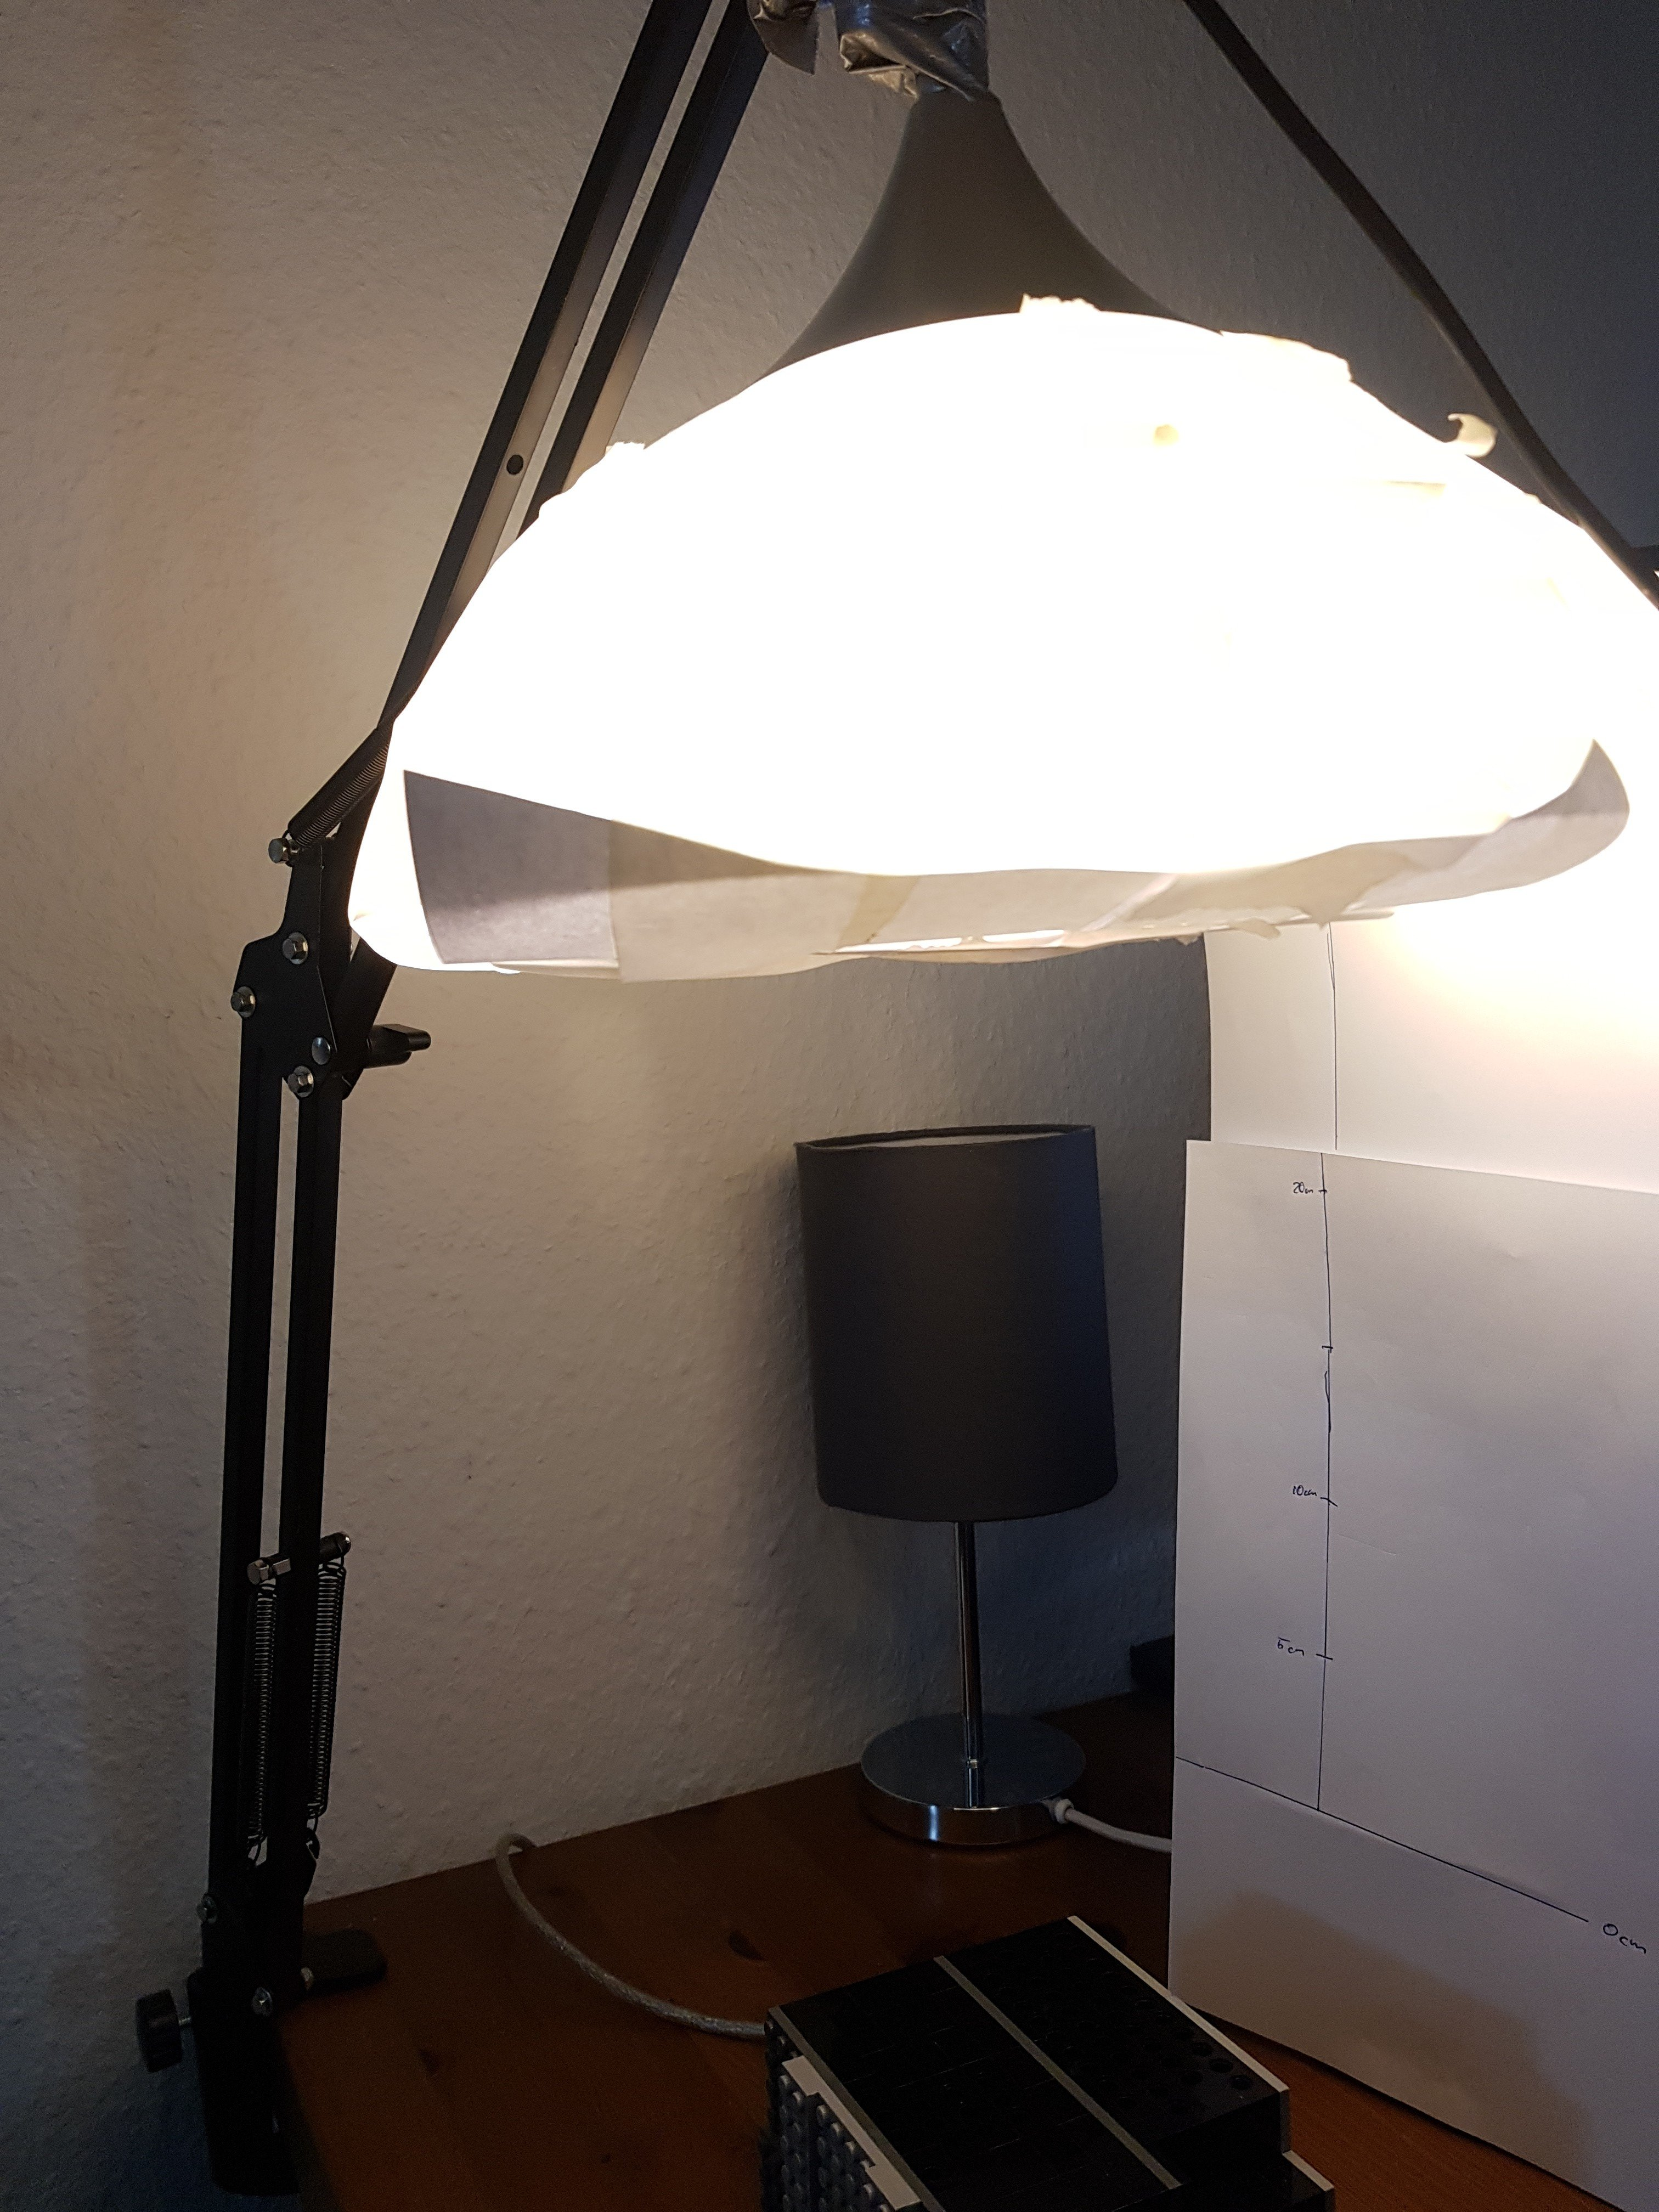
\includegraphics[width=0.33\linewidth]{images/light_low.jpeg}}\hfill%
\subfigure[Halbe Helligkeit]{\label{subfig:light_medium}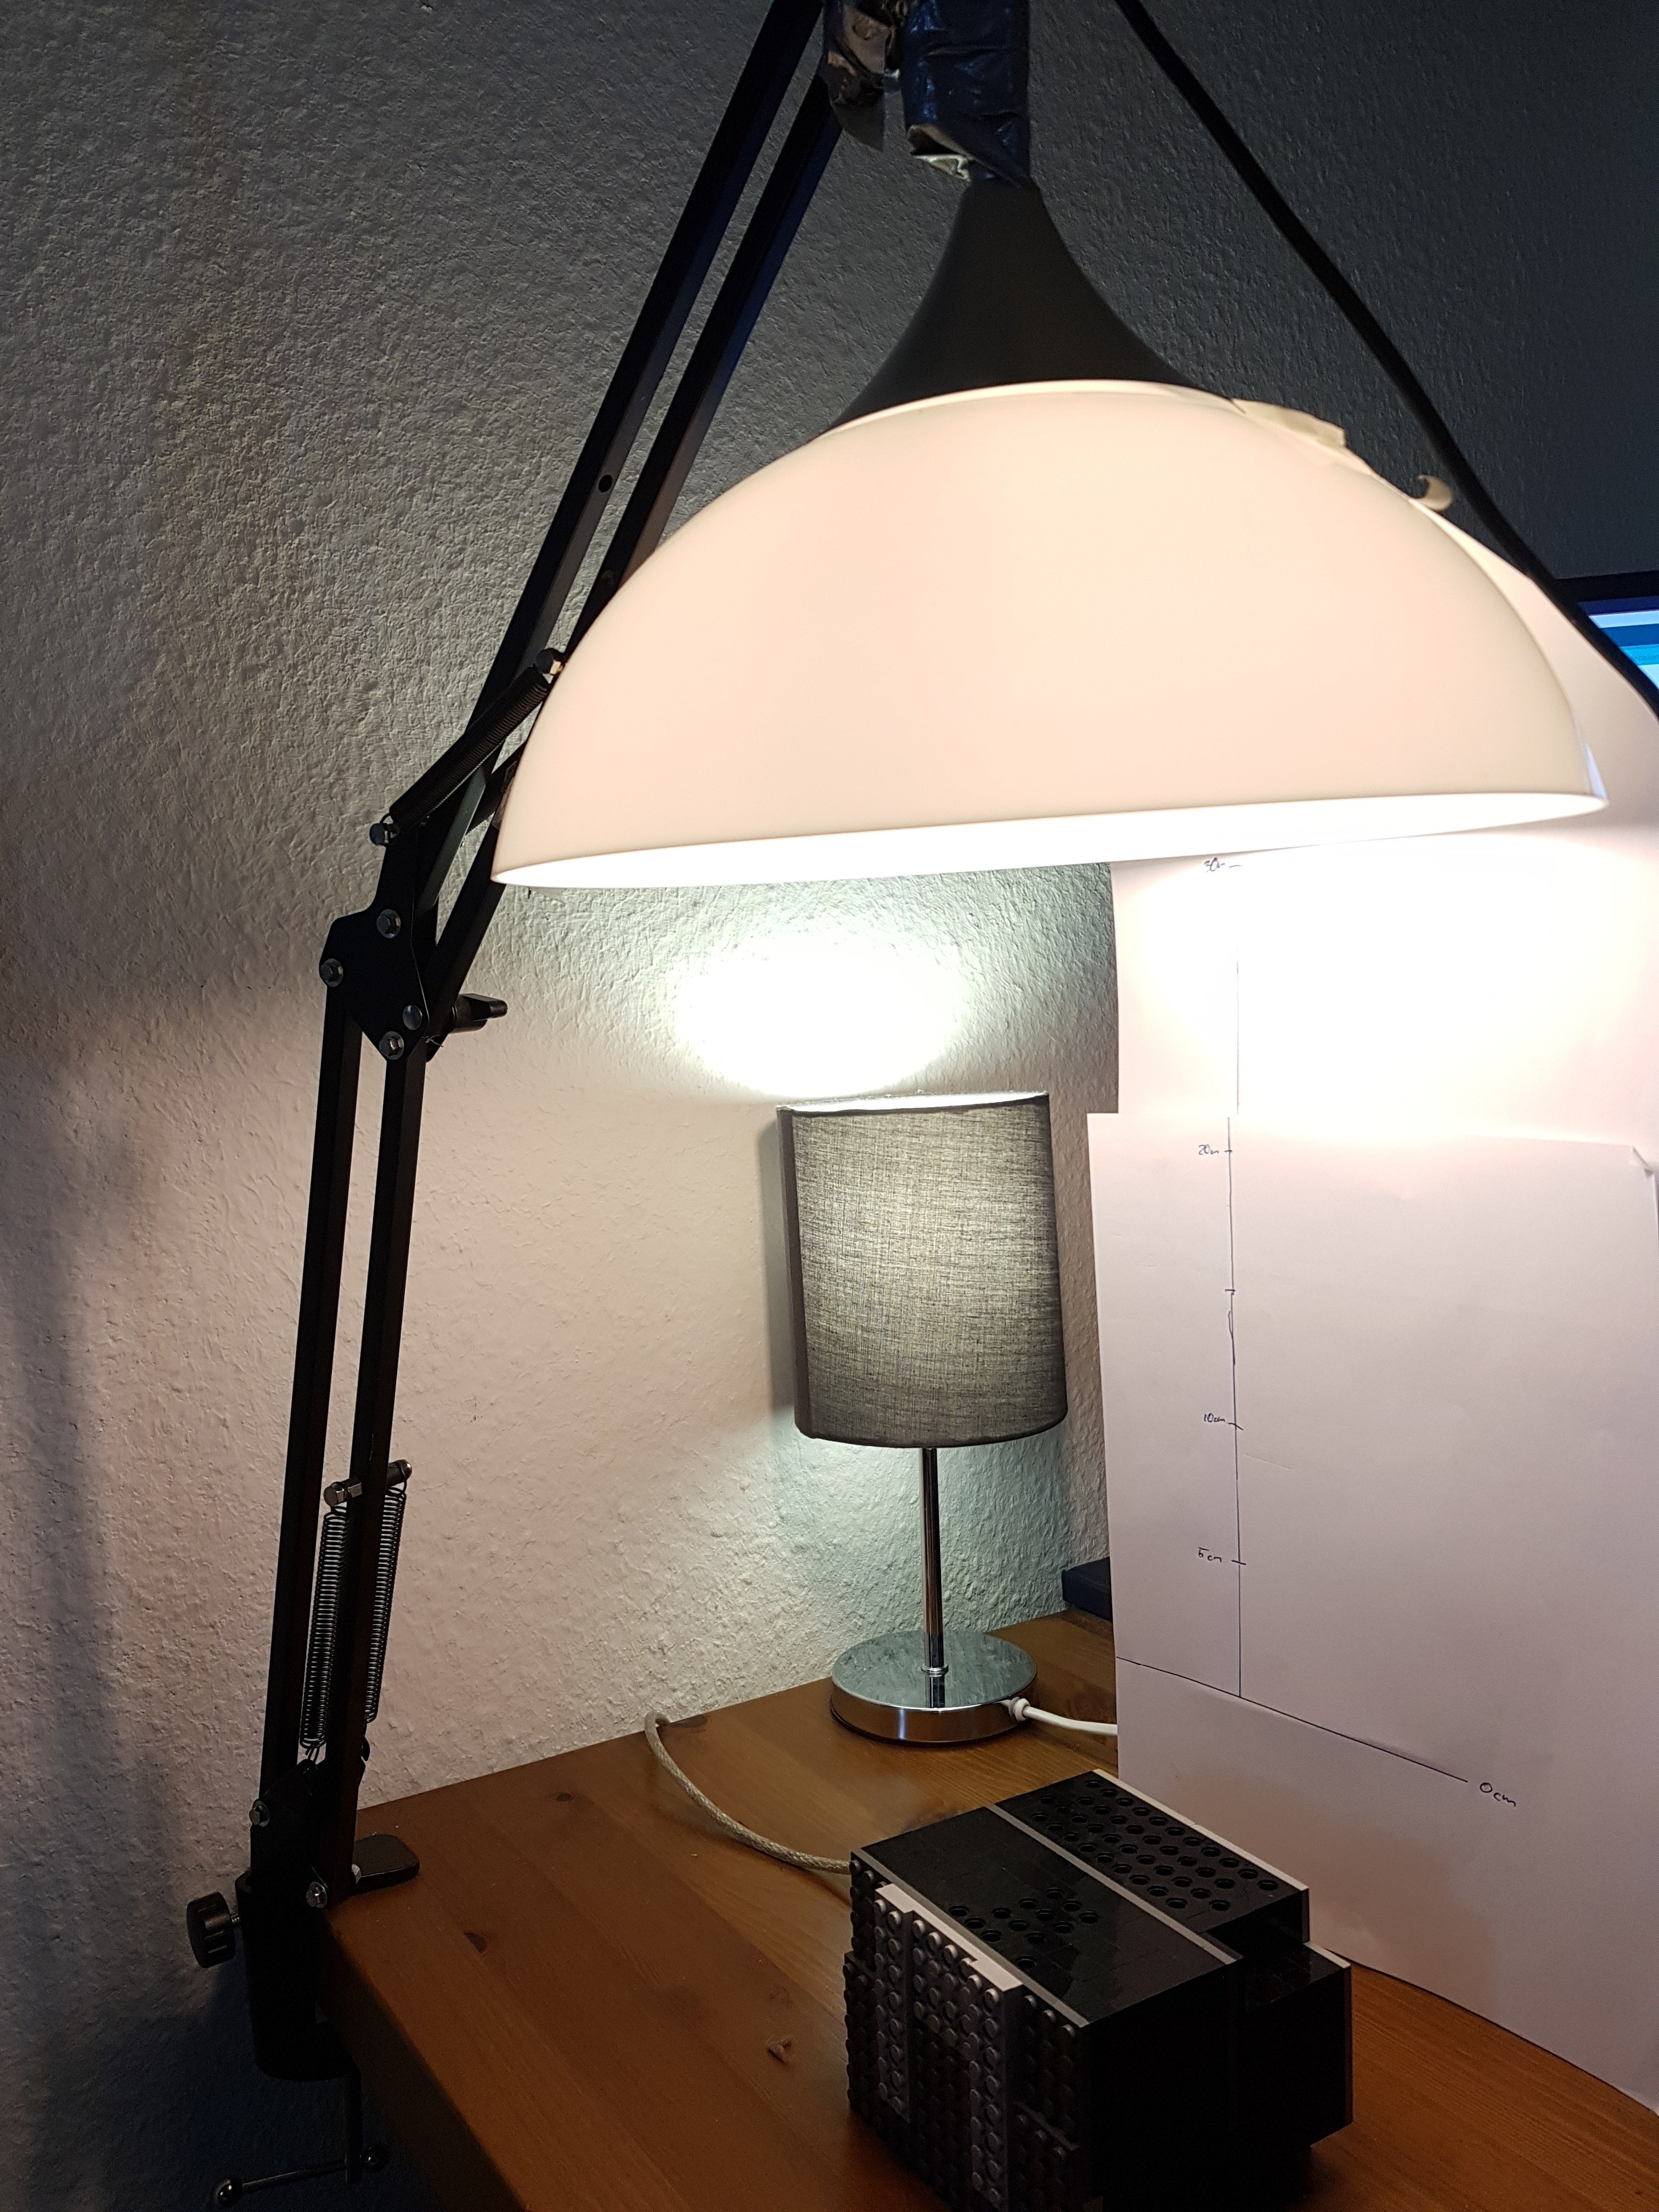
\includegraphics[width=0.33\linewidth]{images/light_medium.jpeg}}\hfill%
\subfigure[Hohe Helligkeit]{\label{subfig:light_high}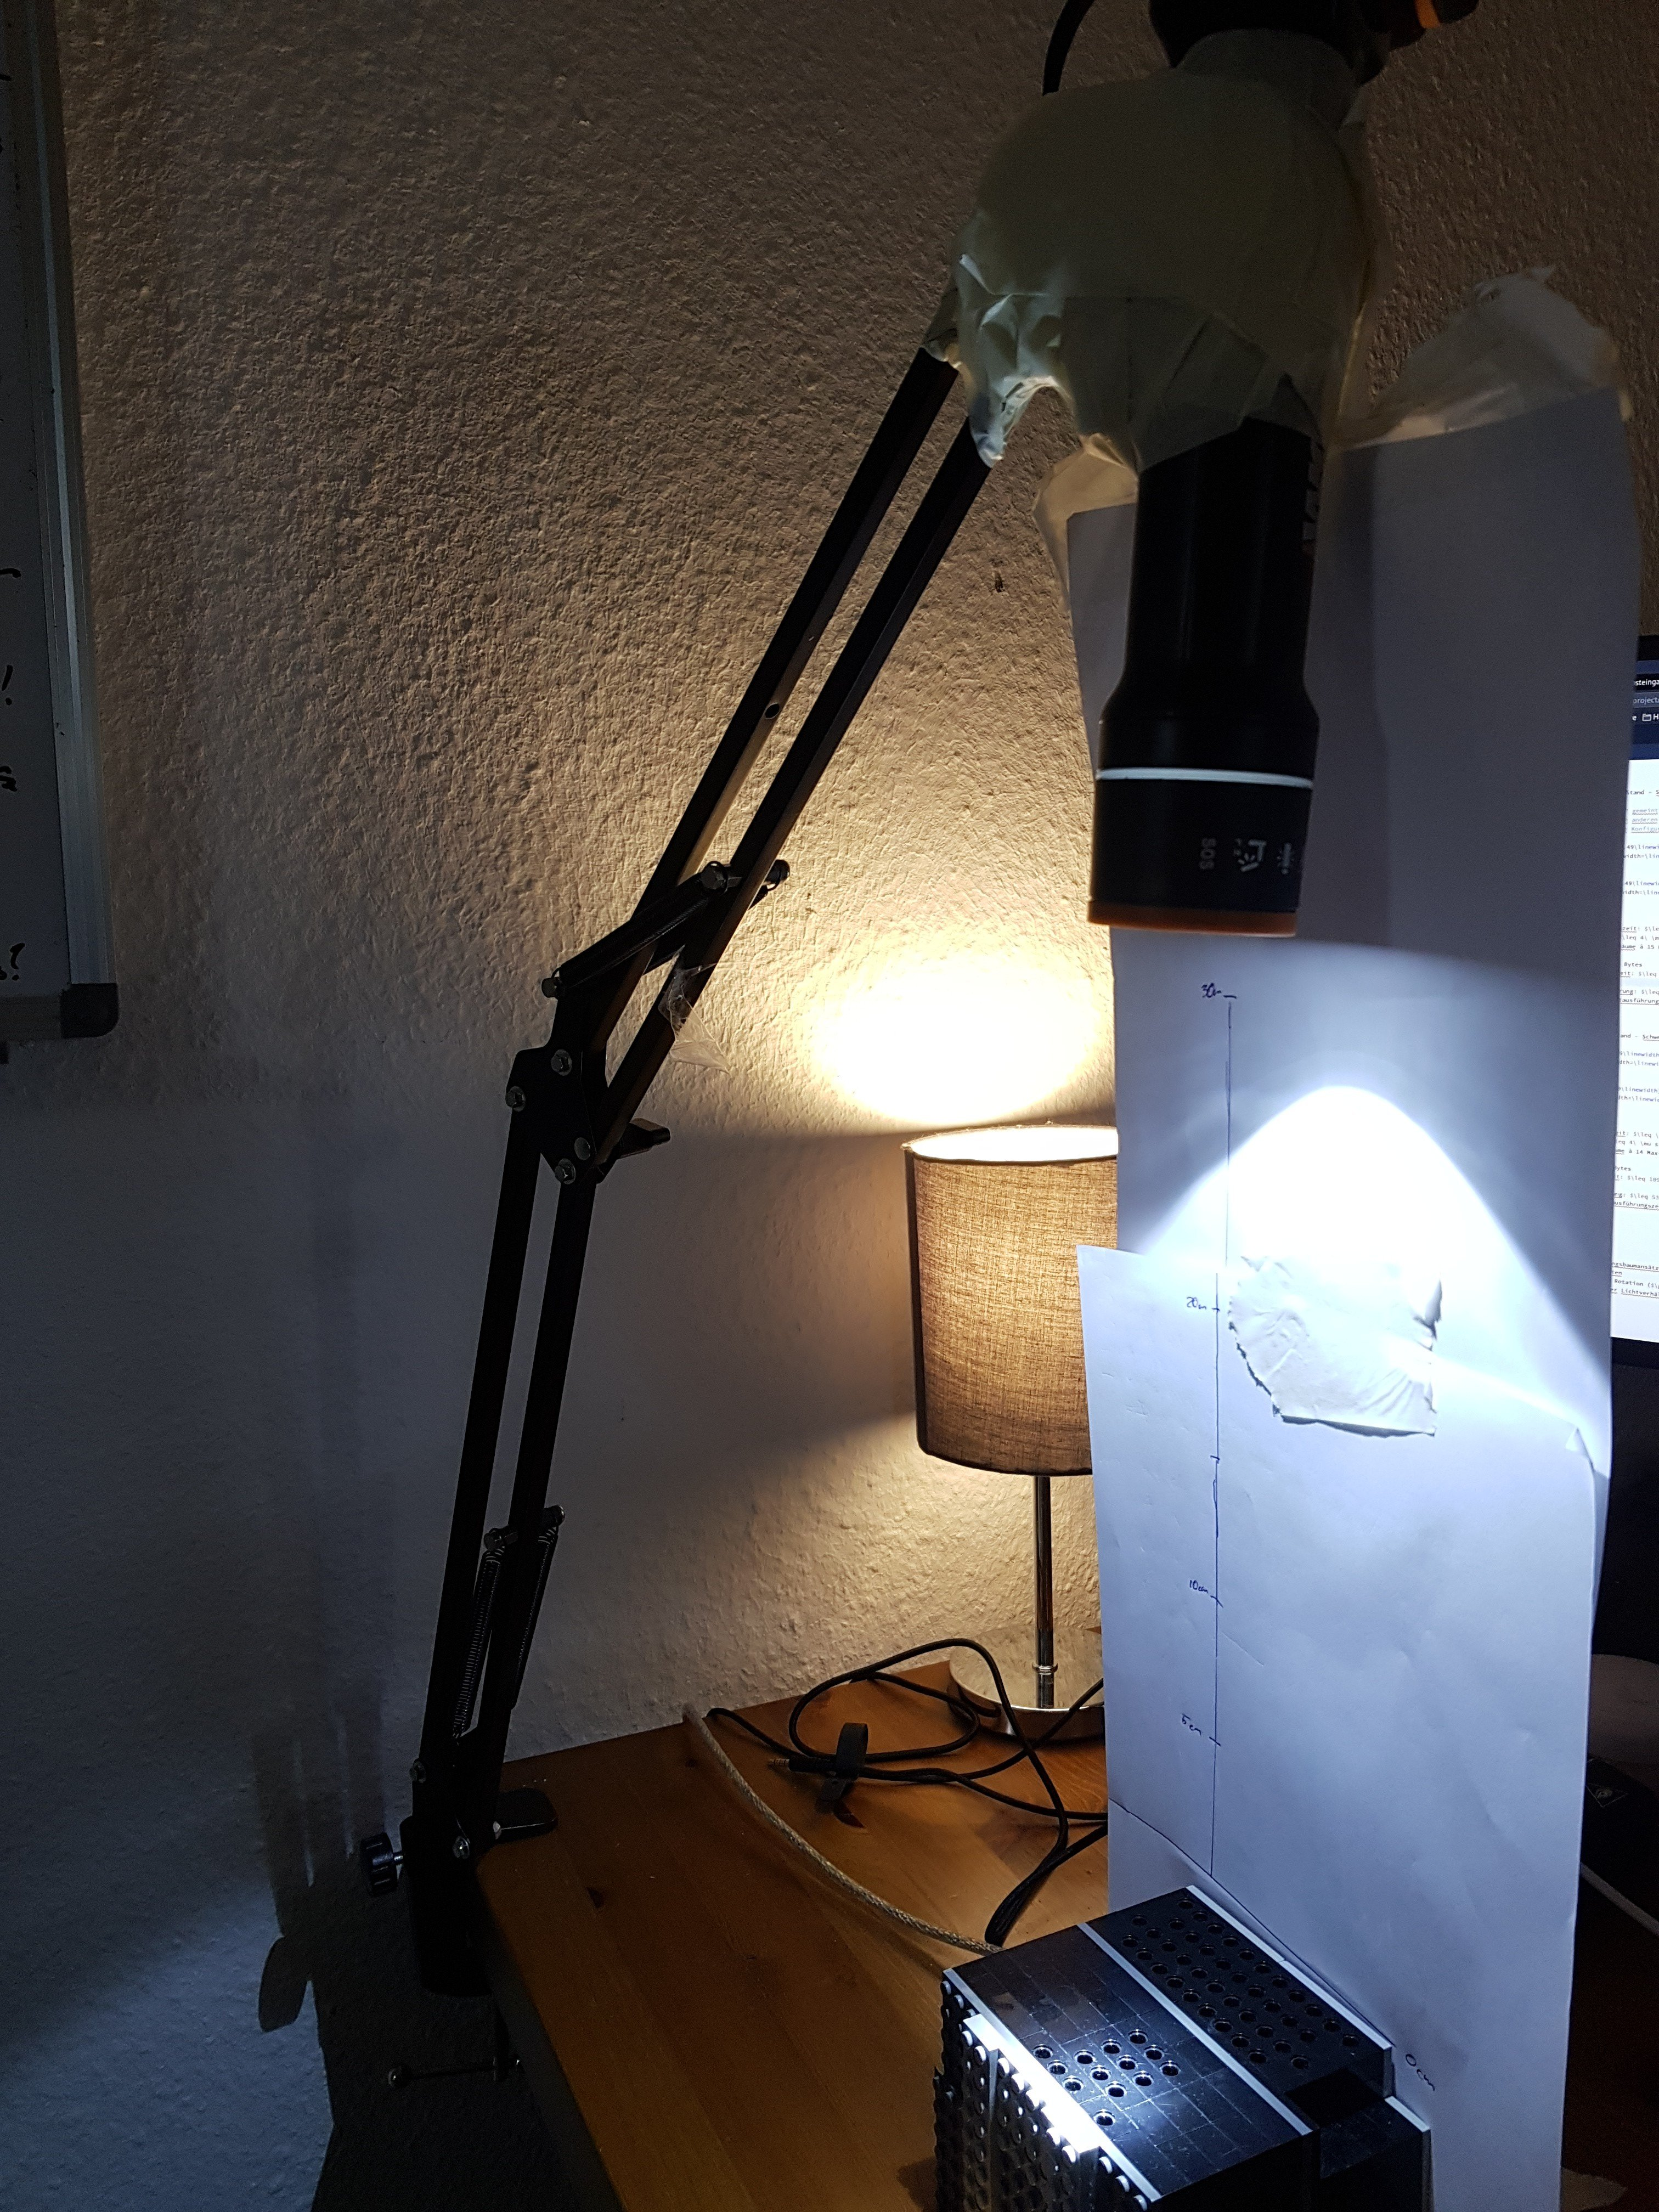
\includegraphics[width=0.33\linewidth]{images/light_high.jpeg}}%
}{Verschiedene Helligkeitsstufen unter denen die Handgesten aufgenommen wurden.}{fig:different_lights}
Es wurden 2 Typen von Nullgesten aufgenommen. Die erste Nullgeste soll eine valide Handgeste ca. zur Hälfte ausführen und dann umkehren. Die aufgenommen Nullgesten gehen dafür \textit{Oben} rein und führen
20\% bis 70\% der Handgeste aus, bevor umgekehrt wird, um \textit{Oben} wieder rauszukommen. Die zweite Nullgeste soll eine Eckbewegung bzw. Kreisbewegung darstellen, indem bei einer Richtung eingedrungen
wird und bei einer benachbarten Richtung ausgetreten wird. Die aufgenommen Nullgesten dafür sind \textit{Oben} rein und führen die valide Handgeste zu 20\% bis 70\% aus, bevor anschließend \textit{Rechts}
ausgetreten wird. Die resultierenden Handgesten werden anschließend um 90°, 180° und 270° rotiert, um die equivalenten Nullgesten aus den anderen Richtungen zu inferieren. Insgesamt entstehen dadurch 19400
Nullgesten. Im weiteren Verlauf dieser Arbeit wird diese Datenmenge mit ausschließlich Nullgesten \glqq Nullgestenmenge\grqq\ genannt. Die ersten 12,5\% werden zum Trainieren verwendet, die hinteren 87,5\% zum
Testen. Die Testmenge wird im weiteren \glqq Nullgestentestmenge\grqq\ genannt.
\newline
\newline
Aus der Gestentestmenge wurden Testmengen erstellt, die testen wie gut ein Modell sich gegenüber unterschiedlichen Lichtverhältnissen generalisiert hat. Die Testmenge \glqq Helligkeitstestmenge 1\grqq\
nutzt den Anteil der Gestentestmenge mit der Helligkeit \glqq Gering\grqq\ und ergänzt jeweils 16 Duplikate der Datenmenge mit einem Offset in der Helligkeit zwischen 0 und 800 und mit einer Skalierung
zwischen 1 und 7. Die Testmenge \glqq Helligkeitstestmenge 2\grqq\ nutzt den Anteil der Gestentestmenge mit der Helligkeit \glqq Halb\grqq\ und ergänzt 19 Duplikate. Diese Duplikate werden in 0,05 Schritten
von 1 bis 0.05 skaliert und die Gesamthelligkeit die dadurch reduziert wird, wird auf alle Pixel in gleichen Teilen addiert. Dadurch ändert sich die Gesamthelligkeit nicht, aber der Kontrast zwischen hellen
und dunklen Pixeln wird gesenkt.